\capitulo{5}{Aspectos relevantes del desarrollo del proyecto}

En este apartado se explicaran todos los aspectos y decisiones que han supuesto un punto importante en el desarrollo del proyecto. Además, se hará mención de aquellos puntos críticos que han llevado a tomar esas decisiones.


\section{Ciclo de vida}
Para este proyecto se hizo uso de la metodología Scrum mencionada anteriormente. El motivo de haber empleado esta metodología y no otra, es la continua entrega de resultados, lo que permite una retroalimentación de los mismos, así como las mejoras a implementar para la siguiente entrega. Es un modelo de trabajo que permite llevar el proyecto al día, evitando así cargas de trabajo mayores en la entrega final del proyecto.

Al principio del proyecto se realizaban \textit{sprints}/reuniones cada dos semanas ya que el proyecto se encontraba en fase de desarrollo. En estas semanas se proponían nuevas funcionalidades a implementar, así como, se revisaban los resultados de las propuestas de anteriores reuniones. A su vez, las tareas a llevar a cabo se anotaban como \textit{issues} en el repositorio de GitHub, todo bajo el control de Zube. Cada \textit{commit} relacionado con la \textit{issue} que se lanzaba a la nube, lo hacia con la referencia a la \textit{issue} que resolvía, con el objetivo de lograr un control de versiones sencillo de comprender.

Posteriormente, una vez finalizado el desarrollo principal, las reuniones tenían lugar cada semana. En estas, se daba una guía de como realizar la documentación completa del proyecto, además de, los pequeños cambios que se debían realizar para mejorar algunos aspectos de PlanLMS.

\section{Tipo de arquitectura}
Para el desarrollo del proyecto se optó por utilizar \textit{Clean Architecture}, patrón utilizado en el diseño software que promueve la mantenibilidad del código, así como la escalabilidad del mismo. Se caracteriza por separar las distintas responsabilidades que componen el proyecto \cite{arquitectura_domain}.

Este patrón se caracteriza por dividir el desarrollo en distintas capas en función de las responsabilidades que cada una aborda. Estas capas son \cite{arquitectura_medium}:
\begin{itemize}
    \item \textbf{Capa de entidades:} alberga los objetos de negocio del dominio, es decir, clases que albergan los datos principales del negocio.
    \item \textbf{Capa de Casos de Uso:} contiene clases que representan acciones de negocio, es decir, contiene la lógica de la aplicación.
    \item \textbf{Capa de adaptadores:} se encarga de convertir los datos del exterior en un formato legible por las capas internas.
    \item \textbf{Capa de Frameworks:} esta capa contiene todo el código relativo a las bibliotecas, \textit{frameworks} y herramientas externas.
\end{itemize}

En el caso de este proyecto, se ha divido el código en los siguientes directorios:
\begin{itemize}
    \item \textbf{\textit{backend}:} contiene toda la lógica de la aplicación.
    \item \textbf{\textit{config}:} contiene todas las configuraciones generales de toda la aplicación, en este caso configuración de temas.
    \item \textbf{\textit{models}:} contiene todas las entidades de negocio.
    \item \textbf{\textit{presentation}:} contiene la interfaz gráfica de la aplicación.
    \item \textbf{\textit{services}:} contiene la lógica que obtiene datos externos al proyecto.
    \item \textbf{\textit{utils}:} contiene recursos útiles para todo el proyecto.
\end{itemize}
La división de responsabilidades se ha realizado de esta forma para facilitar el mantenimiento del código, así como la interpretación del funcionamiento del mismo. Por otra parte, esto favorece que el código pueda escalar en el futuro con nuevas implementaciones.

\section{Almacenamiento de datos}
La aplicación aborda dos métodos para el almacenamiento de datos, estos se usan dependiendo de la funcionalidad.

\subsubsection{Almacenamiento de filtros}
Un punto fuerte que ofrece la aplicación es la posibilidad de filtrar todo el contenido que el usuario desee visualizar. El problema surgía en que estos filtros que el usuario escogía, no eran persistentes, por lo tanto, se plantearon dos posibilidades: almacenarlos en la nube o almacenarlos localmente en el dispositivo del usuario. Se optó por la segunda opción por la comodidad que suponía su implementación, además de que permite al usuario de un dispositivo iniciar sesión con múltiples cuentas y almacenar los filtros de todas ellas.

\subsubsection{Almacenamiento de tareas personales}
La creación de tareas personales por parte del usuario requería del almacenamiento de las mismas. En este caso, se optó por alojarlas en una base de datos en la nube. El motivo de esta decisión reside en que el usuario debería de ser capaz de tener acceso a todas sus tareas desde cualquier dispositivo, ventaja que carece el almacenamiento en local.

\begin{figure}[H]
    \centering
    {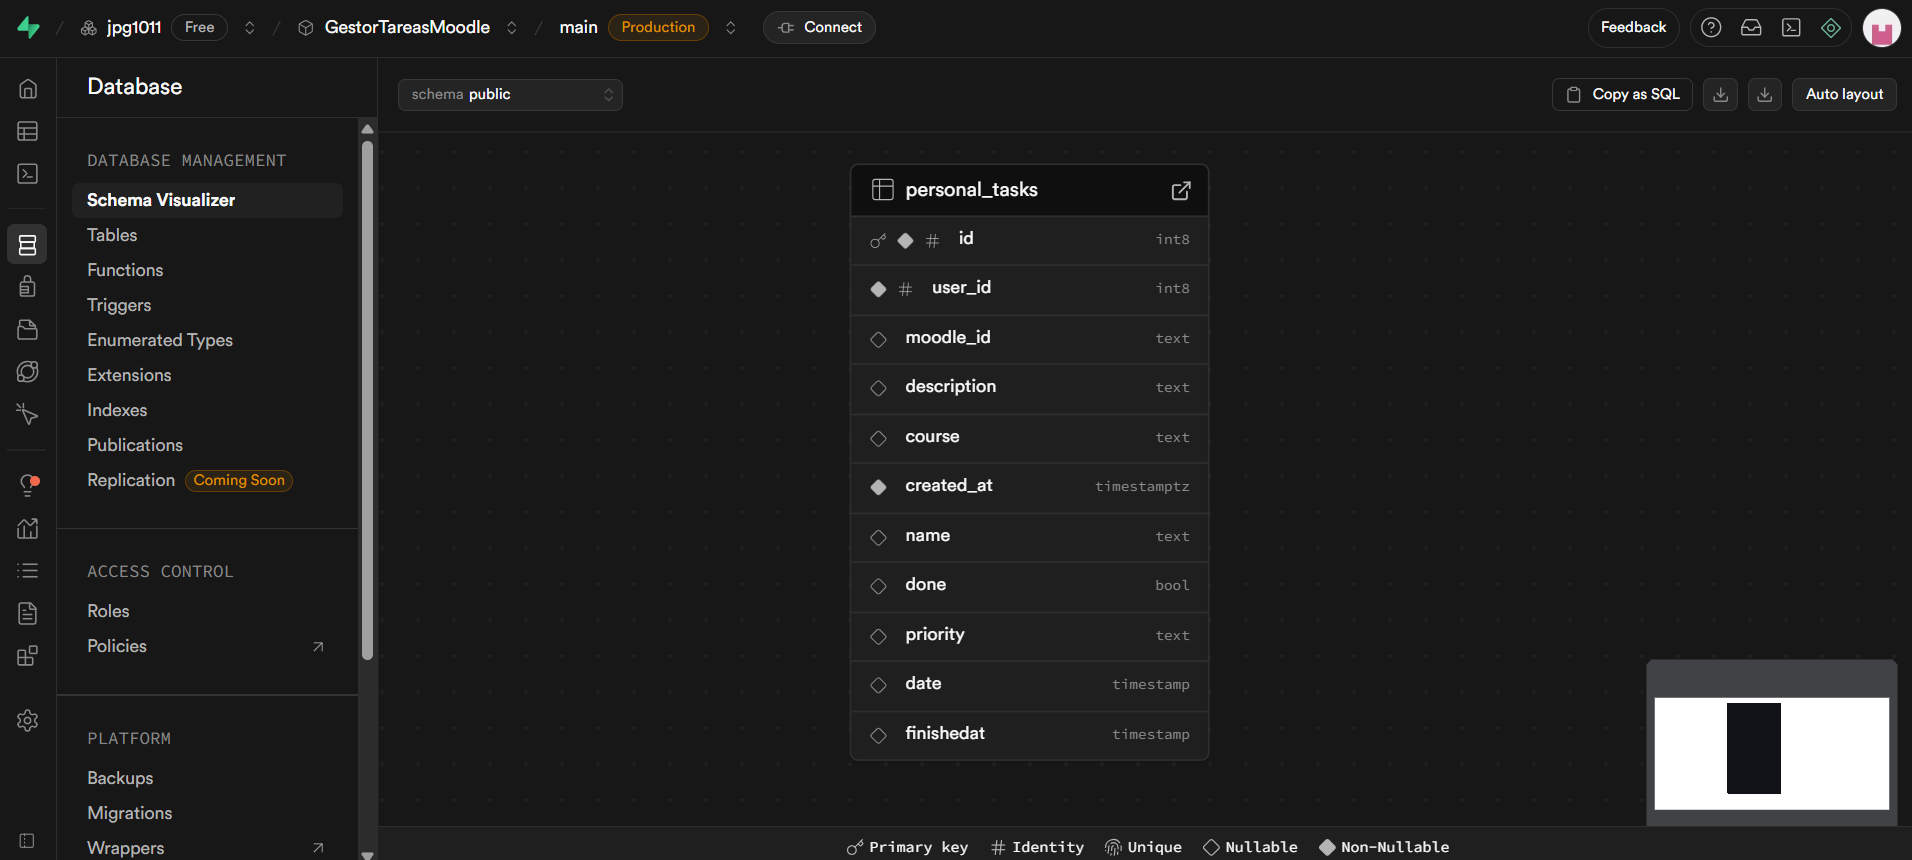
\includegraphics[width=0.8\linewidth]{img/supabase_persistencia.png}}
     {\caption{Dashboard de la base de datos de Supabase}
     \label{fig:supabase_persistencia}}
\end{figure}

\section{Representación de tareas en un diagrama de Gantt}
El diagrama de Gantt representa las tareas de forma que el usuario visualmente puede hacerse a la idea de la duración de dichas tareas. El problema surge cuando existe la ausencia de una de las dos fechas que el diagrama necesita para poder mostrar la duración de las tareas, así como el inicio y el fin de las mismas. En Moodle las tareas y los cuestionarios disponen de una configuración de fechas, pero ese factor depende del responsable que las configure. Por lo tanto, para poder realizar una adaptación de tal forma que se pudieran visualizar las tareas se planteó la asignación de fechas a las tareas en función de qué fechas se disponía. Para entender mejor esto último, se recoge en una tabla la asignación de fechas:

\tablaSmallSinColores
{Fechas disponibles y su respectiva asignación en el diagrama de Gantt}
{cccc}
{disponiblidad-asignacion}
{
    \multicolumn{2}{c}{Disponibilidad}  & \multicolumn{2}{c}{Asignación} \\
    \textbf{Fecha Apertura} & \textbf{Fecha Cierre} & \textbf{Fecha Apertura} & \textbf{Fecha Cierre}\\
}
{
    X & X & Fecha Apertura & Fecha Cierre \\
    X & - & Fecha Apertura & Fecha Apertura \\
    - & X & Fecha Cierre/Actual & Fecha Cierre/Actual\\
    - & - & Fecha Actual & Fecha Actual \\
    
}


En los casos que existen dos posibles fechas para asignar, se realiza una comprobación. Si la fecha de cierre es anterior a la fecha actual, se asigna la fecha de cierre como fecha de apertura. En caso contrario, se asigna la fecha actual. Lo mismo ocurre en el caso de la fecha de cierre.

\begin{figure}[H]
    \centering
    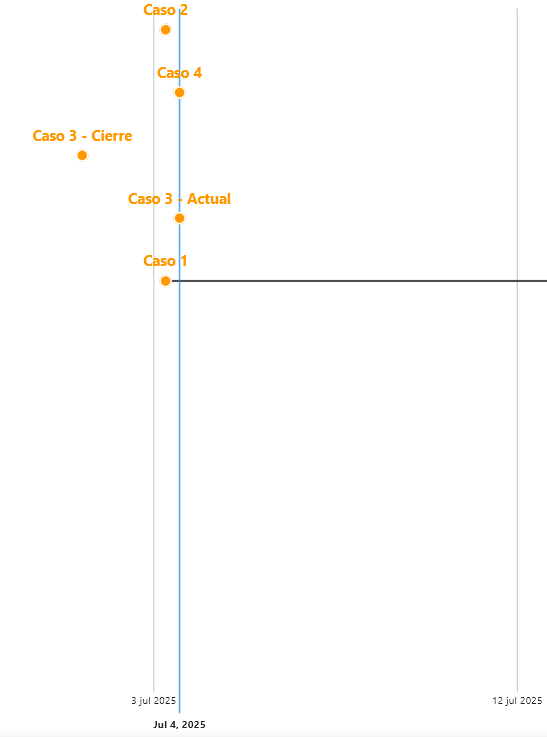
\includegraphics[width=0.7\linewidth]{img/fechas_gantt_ejemplo.png}
    \caption{Ejemplo de la asignación que hace PlanLMS con las fechas}
    \label{fig:fechas_gantt_ejemplo}
\end{figure}

\section{Librería del diagrama de Gantt}
Una vez seleccionada la librería que iba a ser utilizada para la representación del diagrama de Gantt, se puso a prueba con casos prácticos de lo que sería un alumno. En este punto surgieron múltiples problemas:
\begin{itemize}
    \item \textbf{Ausencia de fecha actual:} la visualización del diagrama de Gantt era bastante completa, pero le faltaba un componente muy importante, y era indicar al usuario en qué parte del diagrama se encontrar. Es decir, indicarle en que parte se encontraba la fecha actual, como solución se dibujó una línea azul perpendicular con un texto debajo que muestra la fecha.
    \item \textbf{Definición de alto y ancho:} el diagrama necesitaba una altura y un ancho específico para ser dibujado sobre la pantalla. Cuando se introducía una carga alta de tareas se producían errores que no permitían ver todas las tareas porque el tamaño del diagrama lo limitaba. Como solución se creó una función que calculaba el alto en función del número de tareas que se debían de mostrar. En cuanto al ancho, este puede ser configurado por el usuario a través de los filtros del diagrama.
    \item \textbf{Desajustes generales:} existían algunos desajustes relacionados con la visualización. Algunos desajustes encontrados son:
    \begin{itemize}
        \item Textos cortados por falta de espacio en el diagrama.
        \item Formato de fechas e idioma desconfigurados.
    \end{itemize}

    Todos estos problemas mencionados fueron solucionados modificando el código fuente de la librería del diagrama de Gantt. Como se trata de una modificación, se consultó la licencia, que en este caso es MIT, lo que permitía su modificación y distribución bajo responsabilidad. Posteriormente se alojó localmente la librería con los nuevos cambios que solventaban todos los problemas.
    \item \textbf{Problemas al carecer de tareas:} uno de los primeros problemas encontrados consistía en que al no disponer de tareas para mostrar en el diagrama, se lanzaban errores en la ejecución de la aplicación. Para ello se eliminó la comprobación que limitaba el uso del diagrama sin tareas.
\end{itemize}

\section{Sistema de filtrado}
Como se ha mencionado anteriormente, el sistema de filtrado es uno de los puntos más fuertes de PlanLMS. La idea de hacer un filtro cuyos cambios afecten en toda la aplicación parte de la comodidad de permitir al usuario visualizar el contenido que más le interese, en el momento que desee. El sistema de filtrado se divide en cuatro filtros:
\begin{itemize}
    \item \textbf{Filtrado de cursos:} permite al usuario seleccionar los cursos cuyas actividades o tareas personales quiera visualizar. Por defecto, si no selecciona ningún curso, se mostrarán todos los cursos en los que se encuentre matriculado.
    \item \textbf{Filtrado de tipo de actividad:} existen dos tipos de actividades en el diagrama de Gantt: los cuestionarios y las tareas. Por lo tanto, se permite al usuario seleccionar cual de los dos tipos desea visualizar. Por defecto, se muestran los dos tipos de actividades.
    \item \textbf{Filtrado de fechas:} permite al usuario filtrar las tareas que se encuentren entre un rango de fechas. También se da la posibilidad de seleccionar una de las dos fechas. La ventaja de poder filtrar actividades o tareas personales de esta forma, es que el usuario puede eliminar de su visualización aquellas actividades que ya no se encuentren en su marco temporal.
    \item \textbf{Filtrado de tipo de fecha:} consiste en dos casillas seleccionables que filtran las actividades de Moodle de forma que solo se muestren aquellas que dispongan de una fechas de apertura y de cierre o viceversa. La necesidad de implementar este filtro parte de la ausencia de alguna de estas fechas en la configuración de estas actividades de Moodle.
\end{itemize}

\section{Resolución de errores}
Cuando se planteó el almacenamiento de tareas personales en la nube, la primera opción a implementar fue Firebase. Se realizó la instalación siguiendo la documentación proporcionada por Google Firebase, pero a la hora de realizar la depuración de la aplicación surgió un problema. El compilador indicaba la ausencia de unos ficheros que eran necesarios para poder depurar la aplicación. Se trató de resolver este error, pero la documentación en internet era escasa, por lo tanto, se optó por usar Supabase en sustitución.
